\documentclass[a4paper,12pt,titlepage,portuges]{article}
\usepackage{geometry}       % allows changing page dimensions
\geometry{a4paper,left=2cm,right=2cm,top=2.5cm,bottom=2cm}
\usepackage[latin1]{inputenc}   % support the pt encoding
\usepackage[portuguese]{babel}
\usepackage{graphicx}       % support graphic files
\usepackage{color}          % should allow colored text
\usepackage{url}            % should identify and format urls
\usepackage{natbib}         % pretty bibtex
\usepackage{enumerate}			% allows enumerations a)... I..., 1... etc.
%\usepackage{rotating}				% allows text rotate via \begin{sideways} or \begin{turn}{ang_in_deg}
%\usepackage{lscape}					% allows pages in landspace \begin{landscape}page content\end{landscape}
\usepackage{url}
\usepackage[pdftex,
	pdftitle					= {creating urban scenery using multimodal interfaces},
	pdfauthor					= {Jos� Pedro Dias},
	bookmarks         = true,				% do bookmarks
	bookmarksnumbered = true,				% keep sedtion numbers
%	pdfpagemode       = None,				% start with closed bookmarks
	pdfstartview      = FitH,				% starting view scale
%	pdfpagelayout     = SinglePage,	% one page at a time
	linkcolor					= black,			% links inside the document
	citecolor					= black,			% for cites
%	linkcolor					= blue,				% links inside the document
%	citecolor					= red,				% for cites
%	urlcolor					= green,			% for urls
	colorlinks        = true]{hyperref}
\usepackage[absolute]{textpos}		% allows absolute positioning of stuff

\usepackage{fancyhdr}							% cool headers and footers with \{l,c,h}head and \{l,c,h}foot
\setlength{\headheight}{15pt}
\pagestyle{fancy}
\lhead{Relat�rio de TFC - Urban Sketch}
\rhead{\today}
\lfoot{Jos� Pedro Dias}
\cfoot{}													% tira nr de p�gina do meio do footer
\rfoot{\thepage}


%\usepackage{pict2e}								% these 2 are for table a\b cells
%\usepackage{slashbox}							% pict2e is optional but enhances the result

\usepackage{my-customs}					  % my overloads
%\def\hellow{
%	\textcolor{red}{HELLO!}
%}
%
%% with receiving param
%\def\hellow2#1{
%	\textcolor{red}{begin #1 end}
%}
%
%% alternative way of starting ending a command
%\def\hellow3#1{
%	{\bf#1}
%	\begin{bf}#1\end{bf}
%}

% show TODOs
\def\TODO#1{
	%\glossary{#1}
	\textcolor{red}{\textbf{TODO:} #1}
}

% hide TODOs
%\def\TODO#1{}
										% aliases for common formatting stuff

\title{
	%\TODO{this generates 1 badbox}
	\begin{textblock}{0}(12.5,1)
		
\includegraphics[width=2.5cm]{gfx/logo-ist.jpg}
	\end{textblock}
	\textsc{Relat�rio Intercalar}\\
	\textbf{URBAN SKETCH\\Introdu��o Expedita de Paisagens\\Urbanas via Interfaces Multimodais}
}
\author{
	\textbf{Jos� Pedro Dias}\\
	n.48296\\
	\emph{jose.pedro.dias@gmail.com}
}
\date{Janeiro de 2007}

%\makeindex
%\makeglossary

\begin{document}

\maketitle
%\newpage

\tableofcontents
%\listoffigures
%\listoftables
\newpage

\parskip=0.5\baselineskip

%\twocolumn
	
\baselineskip = 16pt    % bigger space between lines

\section{Introdu��o}
\section{Introdu��o}

O prop�sito deste trabalho � o de permitir a utilizadores a execu��o de opera��es geom�tricas sobre
modelos tridimensionais.
As opera��es devem ser fornecidas ao utilizador de forma contextual, no pr�prio ambiente de visualiza��o,
fornecendo um conjunto de restri��es direccionais de modo a auxili�-lo a obter o efeito desejado.

A aplica��o de uma opera��o inicia-se com a selec��o atrav�s de um tra�o de uma face ou aresta a afectar,
o que despoleta o aparecimento de um menu contextual.
O utilizador escolhe ent�o a opera��o a aplicar, sendo esse mesmo tra�o interpretado para determina��o
dos par�metros da opera��o.

O sistema foi implementado como funcionalidade do prot�tipo multimodal ImmiView presente no laborat�rio Louren�o Fernandes
do IST Tagus Park \cite{leme}, permitindo a sua aplica��o em cen�rios com tablet PCs ou ecr�s de larga escala.

\begin{figure}[!ht]
	\centering
	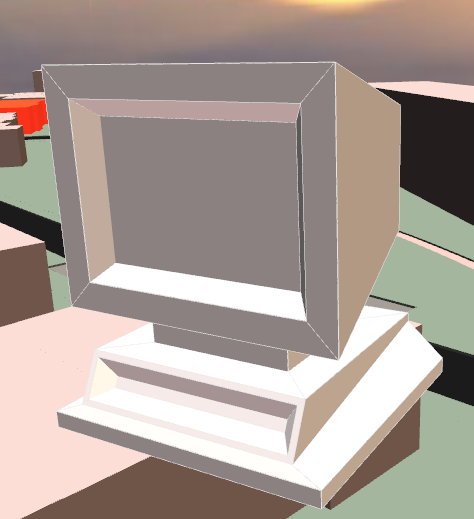
\includegraphics[width=0.4\linewidth]{ex-monitor.png}
	\vspace{-3mm}
	\caption{monitor modelado no sistema}
	\label{fig:example}
	\vspace{-3mm}
\end{figure}

\newpage

\section{Objectivos e Resultados a Obter}
%Nesta sec��o devem descrever brevemente os objectivos a alcan�ar com o vosso trabalho.
%Em rela��o aos Resultados devem ser claros e concisos.
%Em que consistir� o principal resultado do vosso trabalho?
%Como vamos poder saber que os resultados foram alcan�ados?
%Esta � uma sec��o muito importante do vosso relat�rio intercalar. 
%(no m�ximo 1 p�gina)

Este projecto prop�e-se auxiliar um arquitecto no estudo de poss�veis edifica��es.
Est� pensado para ser usado na fase em que o mesmo executa esbo�os, antes da elabora��o
de documentos precisos do mesmo.
Deve ent�o fornecer ferramentas que permitam ao arquitecto desenhar fachadas de edif�cios
e testar a disposi��o dos espa�os de forma pouco precisa.
Esta tarefa deve permitir-lhe tomar decis�es quanto ao futuro tra�ado do edif�cio e
validar com clientes a solu��o alcan�ada.
Num cen�rio de revis�o com clientes ser� ent�o poss�vel a v�rios utilizadores navegar
no mundo, fazer pequenas manipula��es de geometria e apar�ncia (ex: translac��es,
altera��es de material) e gera��o e leitura de anota��es.
Note-se que este cen�rio poder� ocorrer com os utilizadores no mesmo local ou ligados
por rede.

\newpage

\section{Trabalho Relacionado}
%Nesta sec��o deve aparecer a resenha do trabalho relacionado (artigos, autores)
%que j� consultaram, identificando pontos fortes e pontos fracos de cada trabalho,
%no fundo deve ser uma vers�o mais curta do vosso trabalho de Introdu��o � Investiga��o.As refer�ncias devem remeter para a Bibliografia.
%(no m�ximo 10 p�ginas).

!resumo do survey!

\newpage

\section{Trabalho Realizado}
%Descri��o sum�ria do que motivou o trabalho efectuado at� agora. 
%Uma descri��o do trabalho realizado at� agora:
%  An�lise de tarefas,
%  prot�tipos de baixa fidelidade,
%  avalia��es heur�sticas,
%  prot�tipos, etc.
%Em resumo, aqui � onde voc�s mostram que j� trabalharam e
%onde apresentam os principais resultados obtidos. 
%(no m�ximo 1,5 p�ginas).

\TODO{Falta conte�do - ler blog, ver wiki. T�picos manhosos :P}

Este projecto � motivado pela vontade de auxiliar os profissionais do ramo da arquitectura.
Nas �ltimas d�cadas tem sido uma das disciplinas que mais exige dos computadores,
mantendo-se estagnado o modo como o utilizador interage com o software.
Este projecto pretende encontrar formas alternativas de o fazer.
A inclus�o do projecto no cons�rcio Improve � igualmente motivante, estabelecendo um conjunto
de objectivos e prazos adicionais ao projecto.

O projecto teve in�cio no final de Setembro.
Houve uma reuni�o com o cons�rcio Improve, no INESC Lisboa, a que o autor compareceu
e onde se familiarizou com o estado actual de desenvolvimento do projecto, os desafios que
coloca e os prazos e \emph{deliverables} estipulados.

Houve igualmente um conjunto de reuni�es com vista a elucidar os diversos alunos de mestrado quanto
�s tarefas que deles se espera e os prazos a cumprir.

Foi criado um blog \cite{SITE-BLOG} para documentar o desenvolvimento do projecto,
de modo a fornecer aos orientadores uma ferramenta que lhes permita acompanhar o mesmo,
assim como documentar as diversas etapas para uso do autor.

Seguiu-se uma fase de prepara��o para as ferramentas a usar.
Foram executados pequenos programas para ganhar � vontade no uso do OpenSG\footnote{
OpenSG � um grafo de cena que permite um melhor aproveitamento da vertente gr�fica
de um sistema, optimizando a sequ�ncia de chamadas � placa gr�fica e facultando ao
programador classes �teis para o mesmo se abstrair da complexidade do problema.
Este sistema foi escolhido pela \emph{framework} AICI uma vez que permite a distribui��o
da renderiza��o por v�rios n�s.
}\nocite{SITE-OPENSG}
e instalado todo o software necess�rio ao desenvolvimento do projecto, entre ele:

\begin{description}
	\item[Microsoft Visual Studio 2003] --
		como ambiente de compila��o;
	\item[TortoiseSVN] --
		para uso de reposit�rio, permitindo o desenvolvimento colaborativo de software;
	\item[AICI] --
		Trata-se uma \emph{framework} de eventos constru�da em cima do OpenSG.
		Permite receber dados de entrada de diversos dispositivos (rato, caneta, artefactos, etc.)
		e mapear comandos e ac��es a eventos simples ou complexos desses dispositivos,
		facilitando a programa��o em sistemas de t�o complexa interac��o de entrada.
\end{description}

Foram efectuadas diversas reuni�es com o prop�sito de definir objectivos do projecto
e foram escritos casos de uso de modo a estabelecer as funcionalidades suportadas pelo sistema
e sequ�ncias v�lidas de ac��es que permitam efectuar tarefas comuns em cen�rios de arquitectura.

Foi conduzido um levantamento de artigos relevantes no dom�nio do projecto, nas �reas de:
representa��o de geometria complexa (para a robusta visualiza��o de cidades),
interfaces imersivas (para melhor aproveitamento da LemeWall),
interfaces de entrada (para integrar \emph{motion tracking}, reconhecimento de voz, etc.),
interpreta��o de esbo�os,
interfaces sugestivas e restri��es de geometria.

Foi implementado at� ao momento um sistema de gest�o de n�s de geometria,
um gestor de selec��es (suportando \emph{picking} de objectos e selec��o \emph{lasso}).
Foi criada uma interface de selec��o de comandos baseada em gates, inspirada no artigo
\cite{CROSSY}.


\newpage

\section{Trabalho Proposto}
%Com base no trabalho e resultados j� obtidos, descrevam tudo o que ainda est� por fazer,
%de forma devidamente estruturada.
%Isto deve incluir a descri��o de ideias por implementar, a arquitectura dos sistemas
%ou suas componentes que j� estejam definidas nesta altura e os aspectos do sistema que,
%embora ainda n�o 100% concretos, vir�o a ser refinados mais adiante.
%� importante mostrar a utilidade do trabalho anterior onde este for relevante,
%mostrando que as decis�es tomadas para o futuro n�o surgem "do ar".
%(no m�ximo 0,5 p�ginas).

<trab-pro here>

\newpage

\section{Plano de Trabalhos}
%Uma descri��o concreta do trabalho a efectuar at� ao final do projecto,
%com base no vosso cronograma, indicando aspectos concretos do mesmo:
%30 de Janeiro de 2006: xpto xpto xpto xpto xpto
%20 de Fevereiro de 2006: xpto xpto xpto xpto xpto
%N�O SE ESQUE�AM que a escrita do relat�rio final LEVA tempo.
%Incluam pelo menos dois a tr�s meses para esta.
%(no m�ximo 0,5 p�ginas).

\setlength{\columnsep}{0cm}
\begin{multicols}{2}
{\tiny
	\begin{description}
		\item[16 Fevereiro] Prot�tipo Alfa
		\item[13 Mar�o] In�cio dos Testes de Usabilidade
		\item[17 Mar�o] In�cio da escrita do Relat�rio Final
		\item[ 8 Abril] Fim dos Testes de Usabilidade
		\item[27 Abril] Prot�tipo Beta
		\item[29 Maio] Revis�o do Relat�rio Final
		\item[17 Junho] Prot�tipo Final
	\end{description}
}
\vfill{.}

\begin{sideways}
%	\begin{figure}[!h]
		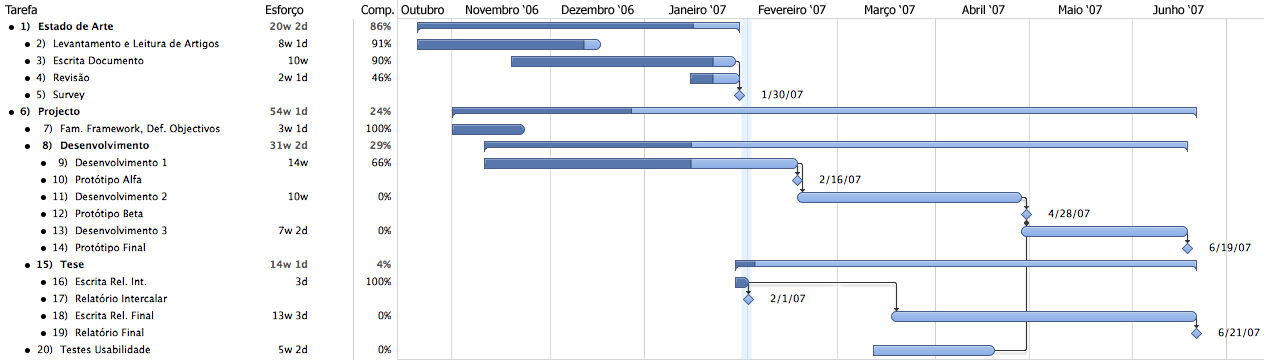
\includegraphics[height=7cm]{gfx/gantt.png}
%	\end{figure}
\end{sideways}
\end{multicols}

\newpage

\section{Conclus�es}
%Apresentar algumas conclus�es em rela��o ao trabalho realizado,
%aos resultados atingidos at� ao momento e ao caminho a seguir a partir de agora. 
%(no m�ximo 0,5 p�ginas).

O levantamento de artigos para a elabora��o do estado de arte permitiu ter uma
melhor no��o de como escrever um artigo.

A aplica��o da interface de gates tem tido resultados satisfat�rios.

Segue-se a conclus�o do primeiro prot�tipo, do qual constar�o funcionalidades de desenho
de primitivas via esbo�os recorrendo a um algoritmo de \emph{curve fitting} que ser� igualmente
desenvolvido.

Assim que estiver dispon�vel um pequeno conjunto de ferramentas, � proveitoso proceder aos
primeiros testes de usabilidade de modo a identificar as maneiras mais eficazes de interagir com o sistema.

%\onecolumn
\newpage

%\bibliographystyle{plain}
\bibliographystyle{alpha}   % this style uses the authors first letters followed by year
\bibliography{thesis}

%\printindex

\end{document}
